% !TEX encoding   = UTF8
% !TEX spellcheck = ru_RU
% !TEX root = ../seminars.tex

%%==================================================
\chapter{Графическое представление функций и данных}
%%==================================================

%%==========================================
\section{Улучшение класса \texttt{Function}}
%%==========================================
Представим вариант выполнения упражения~2 из~\textbookref{главы~15}.

\cppfile[firstline=11, lastline=29]{projects/ch15/function.cpp}

Первый раз основную работу по~вычислению и сохранению точек выполняет конструктор базового класса \code{Function}. Нам остаётся сохранить параметры, задающие вид кривой:

\cppfile[firstline=31, lastline=36]{projects/ch15/function.cpp}

Метод \code{move()} перекрывает \code{Shape::move()}, чтобы сдвинуть начало координат для~правильного вычисления точек кривой, если будут внесены какие-либо дополнительные изменения (форма кривой, диапазон рисования, и т.\,д.):

\cppfile[firstline=38, lastline=43]{projects/ch15/function.cpp}

Следующие функции позволяют пользователю изменить вид кривой:

\cppfile[firstline=45, lastline=64]{projects/ch15/function.cpp}

Основную работу при~этом выполняет закрытая функция \code{redistribute()}, которая вычисляет точки кривой заново:

\cppfile[firstline=66, lastline=75]{projects/ch15/function.cpp}

Заметим, что хранение точек в~классе \code{Shape} (подобно тому, как это делает \code{Graph\_}\-\code{lib::Function}) не~позволяет нам уменьшить их количество. По~этой причине мы не~предоставляем пользователю возможность изменять число точек.

Как и всегда, необходимо протестировать новые возможности, например, так:

\cppfile[firstline=116, lastline=133]{projects/ch15/function.cpp}



%%===================
% !TEX encoding   = UTF8
% !TEX spellcheck = ru_RU
% !TEX root = ../seminars.tex

%%====================================
\section{Функторы или объекты-функции}
%%====================================
Эта тема уже была затронута в~разделе на~странице~\pageref{sect:lambda} в~связи с~обсуждением лямбда-выражений. Кратко вспомним этот материал ещё раз и применим его для~решения небольшой задачки.

\emph{Функтором} называют объекты некоторого класса, в~котором перегружен оператор вызова \code{operator()}. Использование этого оператора синтаксически выглядит как вызов обычной функции. Таким образом, там, где синтаксически требуется вызов функции, можно использовать как простые функции, так и объекты-функции. Например, в~алгоритмах стандартной библиотеки языка~\lang{C++}.

Важные отличия объекта-функции от~обычной функции:
\begin{itemfeature}
  \item можно хранить некоторое состояние и извлекать его после вызова;
  \item количество аргументов можно уменьшить (за~счёт хранения ссылок и данных внутри объекта);
  \item эффективность: часто код функции \code{operator()} короткий и размещается внутри класса. Компилятор делает его подставляемым (\code{inline}). Это редко бывает возможным при~вызове обычной функции через указатель.
\end{itemfeature}



%%==============================================================
\paragraph{Вычисление \(C_n^k\). Динамическое программирование.}
%%==============================================================
Общеизвестная формула для~вычисления количества сочетаний из~\(n\) предметов по~\(k\) штук без~повторений
\[
C_n^k = \frac{n!}{k! (n-k)!}
\]
не~всегда удобна для~расчёта в~программе. Это связано как с~конечностью представления целых чисел, так и с~эффективностью вычислений. Более удобным вариантом может оказаться рекуррентное соотношение
\[
C_n^k = C_{n-1}^{k-1} + C_{n-1}^k,
\]
наглядно вытекающее из~треугольника Паскаля:
\begin{center}
  \begin{tikzpicture}
    \graph [layered layout, level distance=0.5cm]
    {
      n00[as=1];
      n00 -> { n10[as=1], n11[as=1] };

      n10 -> { n20[as=1], n21[as=2] };
      n11 -> { n21,       n22[as=1] };

      n20 -> { n30[as=1], n31[as=3] };
      n21 -> { n31,       n32[as=3] };
      n22 -> { n32,       n33[as=1] };

      n30 -> { n40[as=1], n41[as=4] };
      n31 -> { n41,       n42[as=6] };
      n32 -> { n42,       n43[as=4] };
      n33 -> { n43,       n44[as=1] };

      n40 -> { n50[as=\ldots], n51[as=\ldots] };
      n41 -> { n51,            n52[as=\ldots] };
      n42 -> { n52,            n53[as=\ldots] };
      n43 -> { n53,            n54[as=\ldots] };
      n44 -> { n54,            n55[as=\ldots] };
    };
  \end{tikzpicture}
\end{center}

Если следовать простой идее рекурсии, то есть использовать чистую стратегию <<разделяй и властвуй>> (как, например, поступают в~сортировке слиянием), пришлось бы решать некоторые подзадачи многократно. В~итоге сложность алгоритма будет экспоненциальной, а время получения некоторых значений при~достаточно больших~\(n\) (например, \(n > 40\)) весьма заметным.

Чтобы избежать повторного решения подзадач, следует запоминать полученные ответы и брать их из~таблицы, когда понадобятся в~следующий раз. В~этом и состоит суть идеи \emph{динамического программирования}.

\cppfile[lastline=5]{projects/ch15/combinations.cpp}

Попробуем реализовать эту идею с~использованием функтора.

\cppfile[firstline=7, lastline=18]{projects/ch15/combinations.cpp}
\cppfile[firstline=47, lastline=47]{projects/ch15/combinations.cpp}
\cppfile[firstline=49, lastline=52]{projects/ch15/combinations.cpp}

Отметим, что в~этой реализации простота и изящность рекурсивного алгоритма, рассматриваемого ниже, совмещается с~высокой эффективностью, а детали (таблица \code{cache}) скрыты от~пользователя. Выделение памяти и заполнение таблицы производится по~мере необходимости.

Квалификатор \cppinline/static/, присутствующий в~объявлении константы \code{invalid}, говорит, что данное свойство (поле) принадлежит классу, а не~конкретному объекту. Его можно использовать без~создания какого-либо объекта, обращаясь по~имени класса:

\cpp/Combinations::invalid/

Такой технический приём, когда у~всех объектов класса есть общее свойство, лежит в~основе реализации концепции \textenglish{Singleton}. В~данной же ситуации мы просто помещаем константу внутрь области видимости класса, скрывая её как деталь реализации.

Это объявление является просто объявлением (до~стандарта \lang{C++17}), поэтому нам необходимо определить объект, то есть выделить память для~него в~этом модуле:

\cppfile[firstline=20, lastline=20]{projects/ch15/combinations.cpp}

Рекурсивный алгоритм, следующий приведённому выше рекуррентному соотношению, можно выразить следующим образом:

\cppfile[firstline=33, lastline=45]{projects/ch15/combinations.cpp}

\noindent Выделяя память, мы инициализируем внутренние элементы некоторым некорректным значением, а на~границах заполняем сразу единицами.

\cppfile[firstline=22, lastline=31]{projects/ch15/combinations.cpp}

%%===================



%%==========================================
\section{Визуализация данных. Аппроксимация}
%%==========================================
В~самом начале мы разбирали метод наименьших квадратов (см.~страницу~\pageref{sect:leastsquares}) для~аппроксимации массива экспериментальных данных. По~аналогии с~материалом \textbookref{главы~15} представим эти данные графически, а также нанесём на график кривые, аппроксимирующие их.

В~качестве реализации метода наименьших квадратов возьмём ранее написанный код. Разместим его в~файлах \code{least\_squares.h} и \code{least\_squares.cpp}. Функции и классы поместим в~отдельное пространство имён \code{lsm}.

Приведём лишь ключевые моменты кода (файл \code{main.cpp}), выполняющего визуализацию. Размеры и положение окна, осей, масштабирующие множители и прочее предлагаем определить самостоятельно, опираясь на~материал учебника.

Добавление данных в~виде точек, отмеченных маркером:

\cppfile[firstline=85, lastline=89]{projects/ch15/least_squares/main.cpp}

\noindent Переменные \code{xs} и \code{ys} "--- объекты класса \code{Scale}, описанного в~\textbookref{главе~15}.

Добавление прямой, коэффициенты которой получены методом наименьших квадратов по исходным данным (из~файла \code{data.txt}):

\cppfile[firstline=94, lastline=104]{projects/ch15/least_squares/main.cpp}

Отметим, что в~регрессионной модели (\ref{eq:linearmodel}) рассмотрен частный случай \(f(x_i) = x_i\). Однако все рассуждения и приведённые выкладки остаются справедливыми и в~том случае, если функция \(f(x_i)\) не~является линейной. Поэтому мы внесли небольшую модификацию в~\code{least\_squares()}, добавив функцию как параметр (файл \code{least\_squares.h}):

\cppfile[firstline=45, lastline=45]{projects/ch15/least_squares/least_squares.h}
\cppfile[firstline=54, lastline=54]{projects/ch15/least_squares/least_squares.h}

Функция \code{linear()} задаёт линейную базисную функцию \(f(x_i) = x_i\), протягивая ниточку к~начальной реализации (\code{main.cpp}):

\cppfile[firstline=14, lastline=14]{projects/ch15/least_squares/main.cpp}

\begin{figure}[h]
    {\centering
        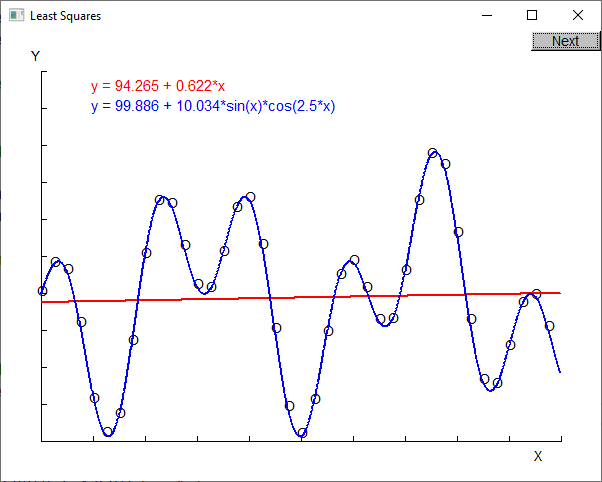
\includegraphics[width=0.6\textwidth]{images/least_squares_graphing.png}

    }
    \caption{Графическое представление данных}
\end{figure}

Вспомогательная функция \code{make\_regression()} создаёт лямбда-выражение, вычисляющее точки аппроксимирующей кривой. При~этом коэффициенты \(a\) и \(b\) скрыты в~реализации объекта лямбда-выражения:

\cppfile[firstline=26, lastline=29]{projects/ch15/least_squares/main.cpp}

Добавьте подпись кривой на~график "--- уравнение модели с~вычисленными коэффициентами. Далее, по аналогии добавьте модель с~нелинейной базисной функцией.



%%================
\WhatToReadSection
%%================
\textcite{Stroustrup:2016:ru}: \textbf{глава~16}



%%===============
\ExercisesSection
%%===============
\begin{exercise}
\item Выполните упражнения из \textbookref{главы~15} учебника.

\end{exercise}
